\documentclass[tikz, border=10pt]{standalone}
\usepackage{tikz}
\usepackage{pgfplots}
\usepackage{siunitx}
\pgfplotsset{compat=1.18}
\usetikzlibrary{arrows.meta, decorations.pathreplacing, calc, positioning}

% ── NACA 4412 profile coordinates (x/c, y/c) ─────────────────────────────────
% Upper surface (leading edge → trailing edge)
% Lower surface (leading edge → trailing edge)
% Scaled by chord C=8cm for the diagram

\begin{document}
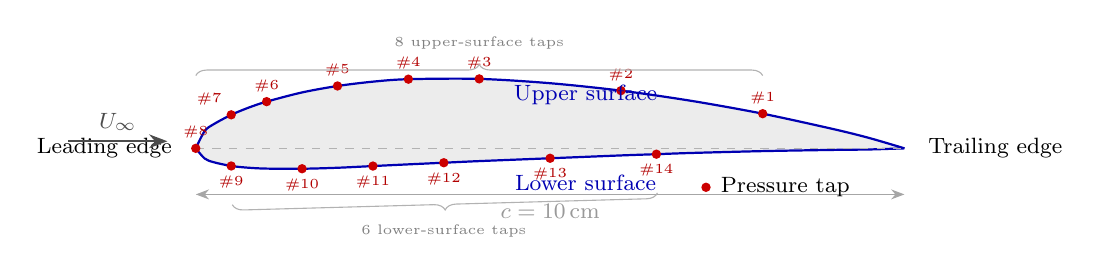
\begin{tikzpicture}[
    scale=9,          % chord = 1 unit → 9 cm on page
    >=Stealth,
    font=\small,
    tap/.style={circle, fill=red!80!black, inner sep=1.2pt},
    label style/.style={font=\footnotesize},
]

% ── Airfoil profile points (NACA 4412) ───────────────────────────────────────
% Upper surface
\def\uppersurf{
    (0,0)
    (0.0125, 0.0244)
    (0.025,  0.0339)
    (0.05,   0.0473)
    (0.075,  0.0576)
    (0.10,   0.0659)
    (0.15,   0.0789)
    (0.20,   0.0880)
    (0.25,   0.0941)
    (0.30,   0.0976)
    (0.40,   0.0980)
    (0.50,   0.0919)
    (0.60,   0.0814)
    (0.70,   0.0669)
    (0.80,   0.0489)
    (0.90,   0.0271)
    (0.95,   0.0147)
    (1.0,    0)
}
% Lower surface
\def\lowersurf{
    (0,0)
    (0.0125,-0.0143)
    (0.025, -0.0195)
    (0.05,  -0.0249)
    (0.075, -0.0274)
    (0.10,  -0.0286)
    (0.15,  -0.0288)
    (0.20,  -0.0274)
    (0.25,  -0.0250)
    (0.30,  -0.0226)
    (0.35,  -0.0203)
    (0.40,  -0.0180)
    (0.50,  -0.0140)
    (0.60,  -0.0100)
    (0.65,  -0.00825)
    (0.70,  -0.0065)
    (0.80,  -0.0039)
    (0.90,  -0.0022)
    (0.95,  -0.0016)
    (1.0,    0)
}

% ── Draw filled airfoil ───────────────────────────────────────────────────────
\fill[gray!15] plot[smooth] coordinates \uppersurf
               -- plot[smooth, ] coordinates {
                   (1.0, 0)
                   (0.95,-0.0016)(0.90,-0.0022)(0.80,-0.0039)(0.70,-0.0065)
                   (0.65,-0.00825)(0.60,-0.0100)(0.50,-0.0140)(0.40,-0.0180)
                   (0.35,-0.0203)(0.30,-0.0226)(0.25,-0.0250)(0.20,-0.0274)
                   (0.15,-0.0288)(0.10,-0.0286)(0.075,-0.0274)(0.05,-0.0249)
                   (0.025,-0.0195)(0.0125,-0.0143)(0,0)
               } -- cycle;

\draw[thick, blue!70!black] plot[smooth] coordinates \uppersurf;
\draw[thick, blue!70!black] plot[smooth] coordinates {
    (0,0)(0.0125,-0.0143)(0.025,-0.0195)(0.05,-0.0249)(0.075,-0.0274)
    (0.10,-0.0286)(0.15,-0.0288)(0.20,-0.0274)(0.25,-0.0250)(0.30,-0.0226)
    (0.35,-0.0203)(0.40,-0.0180)(0.50,-0.0140)(0.60,-0.0100)(0.65,-0.00825)
    (0.70,-0.0065)(0.80,-0.0039)(0.90,-0.0022)(0.95,-0.0016)(1.0,0)
};

% ── Chord line ────────────────────────────────────────────────────────────────
\draw[gray!60, dashed, thin] (0,0) -- (1,0);

% ── Pressure tap markers ──────────────────────────────────────────────────────
% Upper surface taps
\node[tap] (u1) at (0.80, 0.0489) {};
\node[tap] (u2) at (0.60, 0.0814) {};
\node[tap] (u3) at (0.40, 0.0980) {};
\node[tap] (u4) at (0.30, 0.0976) {};
\node[tap] (u5) at (0.20, 0.0880) {};
\node[tap] (u6) at (0.10, 0.0659) {};
\node[tap] (u7) at (0.05, 0.0473) {};
\node[tap] (u8) at (0.00, 0.0000) {};  % leading edge stagnation

% Lower surface taps
\node[tap] (l1) at (0.05,  -0.0249)  {};
\node[tap] (l2) at (0.15,  -0.0288)  {};
\node[tap] (l3) at (0.25,  -0.0250)  {};
\node[tap] (l4) at (0.35,  -0.0203)  {};
\node[tap] (l5) at (0.50,  -0.0140)  {};
\node[tap] (l6) at (0.65,  -0.00825) {};

% ── Tap labels: upper surface (above) ─────────────────────────────────────────
\node[above, font=\tiny, text=red!70!black] at (u8) {\#8};
\node[above left, font=\tiny, text=red!70!black] at (u7) {\#7};
\node[above, font=\tiny, text=red!70!black] at (u6) {\#6};
\node[above, font=\tiny, text=red!70!black] at (u5) {\#5};
\node[above, font=\tiny, text=red!70!black] at (u4) {\#4};
\node[above, font=\tiny, text=red!70!black] at (u3) {\#3};
\node[above, font=\tiny, text=red!70!black] at (u2) {\#2};
\node[above, font=\tiny, text=red!70!black] at (u1) {\#1};

% ── Tap labels: lower surface (below) ─────────────────────────────────────────
\node[below, font=\tiny, text=red!70!black] at (l1) {\#9};
\node[below, font=\tiny, text=red!70!black] at (l2) {\#10};
\node[below, font=\tiny, text=red!70!black] at (l3) {\#11};
\node[below, font=\tiny, text=red!70!black] at (l4) {\#12};
\node[below, font=\tiny, text=red!70!black] at (l5) {\#13};
\node[below, font=\tiny, text=red!70!black] at (l6) {\#14};

% ── Annotations ───────────────────────────────────────────────────────────────
% Leading edge label
\node[left, font=\footnotesize] at (-0.02, 0) {Leading edge};

% Trailing edge label
\node[right, font=\footnotesize] at (1.02, 0) {Trailing edge};

% Chord arrow
\draw[<->, gray!70] (0, -0.065) -- (1, -0.065)
    node[midway, below, font=\footnotesize, gray!80] {$c = \SI{10}{\centi\metre}$};

% Upper/lower surface labels
\node[blue!70!black, font=\footnotesize] at (0.55,  0.075) {Upper surface};
\node[blue!70!black, font=\footnotesize] at (0.55, -0.048) {Lower surface};

% Freestream arrow
\draw[->, thick, black!70] (-0.18, 0.01) -- (-0.04, 0.01)
    node[midway, above, font=\footnotesize] {$U_\infty$};

% Tap legend
\node[tap, label={[font=\footnotesize]right:Pressure tap}] at (0.72, -0.055) {};

% ── Brace: upper taps ─────────────────────────────────────────────────────────
\draw[decorate, decoration={brace, amplitude=4pt, raise=14pt},
      gray!60]
    (0.00, 0.0480) -- (0.80, 0.0480)
    node[midway, above=20pt, font=\tiny, gray] {8 upper-surface taps};

\draw[decorate, decoration={brace, amplitude=4pt, raise=14pt, mirror},
      gray!60]
    (0.05, -0.0249) -- (0.65, -0.0083)
    node[midway, below=20pt, font=\tiny, gray] {6 lower-surface taps};

\end{tikzpicture}
\end{document}
